\documentclass[fleqn]{article}
\usepackage{amsmath}
\usepackage[dvips]{graphicx}
\bibliographystyle{plain}
%__________________________________
\begin{document}

\section*{\center Crushing a Foam Microstructure}
\subsection*{\underline{Problem Description}}
This calculation demonstrates two important strength of MPM.  The first
is the ability to quickly generate a computational representation of
complex geometries.  The second is the ability of the method to handle
large deformations, including self contact.

In particular, in this calculation a small sample of foam, the geometry
for which was collected using microCT, is represented via material points.
The sample is crushed to 87.5\% compaction through the use of a rigid plate, which
acts as a constant velocity boundary condition on the top of the sample.  This
calculation is a small example of those described in \cite{brydonfoam}.  The
geometry of the foam is created by image procesing the CT data, and based
on the intensity of each voxel in the image data, the space represented
by that voxel either recieves a particle with the material properties of the
foam's constituent material, or is left as void space.  This particle
representation avoids the time consuming steps required to build a suitable
unstructured mesh for this very complicated geometry.
 
\subsection*{\underline{Simulation Specifics}}
\begin{description} 
\item [Component used:] \hfill MPM
\item [Input file name:] \hfill foam.ups
\item [Instruction to run input file:]

First, copy foam.ups and foam.pts.gz to the same directory as sus.
Adjust the number of patches in the ups file based on
the number of processors available to you for this run.
Uncompress the pts file {\bf gunzip foam.pts.gz}.

The command:  {\bf pfs foam.ups} will divide the foam.pts
file, which contains the geometric description of the foam,
into number of patches smaller files, named foam.pts.0,
foam.pts.1, etc.  This is done so that for large simulations,
each processor is only reading that data which it needs, and
prevents the thrashing of the file system that would occur
if each processor needed to read the entire pts file.  This
command only needs to be done once, or anytime the patch
distibution is changed.  Note that this step must be done even
if only one processor is available.

To run this simulation:  {\bf mpirun -np NP sus foam.ups}
where NP is the number of processors being used.

\item [Simulation Domain:]\hfill  0.2 X 0.2 X 0.2125 mm

\item [Number of Computational Cells:]\hfill \\ 
102 X 102 X 85 (Level 0)

\item [Example Runtimes:] \hfill \\
 3 hours  (32 processors, 2.4 GHz Xeon)\\
 11 hours (2 processors,  3.0 GHz Xeon)\\

\item [Physical time simulated:] \hfill 3.75 seconds

\item [Associate scirun network:] \hfill foam.srn

\end{description}

\section*{\underline{Results}}

Figure~\ref{figfoam} shows a snapshot of the simulation, as the foam
is at 50\% compaction.
\begin{figure}[b]
  \center
%  \scalebox{0.2}{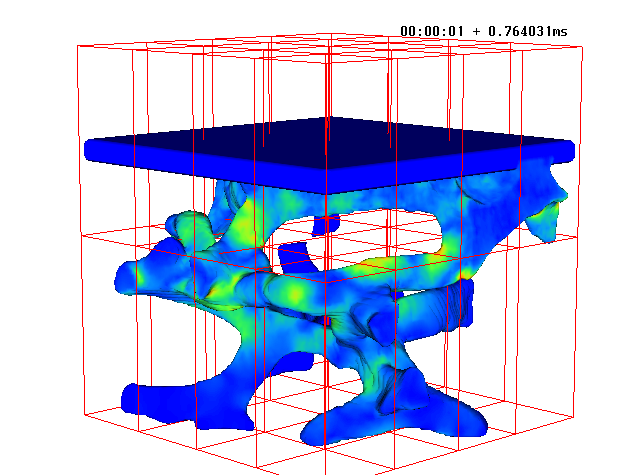
\includegraphics{foam.png}}
  \caption{Compaction of a foam microstructure.}
  \label{figdisks}
\end{figure}

In this simulation, the reaction forces at 5 of the 6 computational boundaries
are also recorded and can be viewed using a simple plotting package such
as gnuplot.  At each timestep, the internal force at each of the boundaries
is accumulated and stored in ``dat" files within the uda,
e.g. BndyForce\_zminus.dat.  Because the reaction force is a vector, it
is enclosed in square brackets which may be removed by use of a script in
the inputs directory:

cd foam.uda.000
../scripts/removeBraces BndyForce\_zminus.dat
gnuplot
gnuplot> plot "BndyForce\_zminus.dat" using 1:4
gnuplot> quit

These reaction forces are similar to what would be measured on a mechanical
testing device, and help to understand the material behavior.

\bibliography{../references}

\end{document}
